\documentclass{article}\usepackage[]{graphicx}\usepackage[]{color}
%% maxwidth is the original width if it is less than linewidth
%% otherwise use linewidth (to make sure the graphics do not exceed the margin)
\makeatletter
\def\maxwidth{ %
  \ifdim\Gin@nat@width>\linewidth
    \linewidth
  \else
    \Gin@nat@width
  \fi
}
\makeatother

\definecolor{fgcolor}{rgb}{0.345, 0.345, 0.345}
\newcommand{\hlnum}[1]{\textcolor[rgb]{0.686,0.059,0.569}{#1}}%
\newcommand{\hlstr}[1]{\textcolor[rgb]{0.192,0.494,0.8}{#1}}%
\newcommand{\hlcom}[1]{\textcolor[rgb]{0.678,0.584,0.686}{\textit{#1}}}%
\newcommand{\hlopt}[1]{\textcolor[rgb]{0,0,0}{#1}}%
\newcommand{\hlstd}[1]{\textcolor[rgb]{0.345,0.345,0.345}{#1}}%
\newcommand{\hlkwa}[1]{\textcolor[rgb]{0.161,0.373,0.58}{\textbf{#1}}}%
\newcommand{\hlkwb}[1]{\textcolor[rgb]{0.69,0.353,0.396}{#1}}%
\newcommand{\hlkwc}[1]{\textcolor[rgb]{0.333,0.667,0.333}{#1}}%
\newcommand{\hlkwd}[1]{\textcolor[rgb]{0.737,0.353,0.396}{\textbf{#1}}}%
\let\hlipl\hlkwb

\usepackage{framed}
\makeatletter
\newenvironment{kframe}{%
 \def\at@end@of@kframe{}%
 \ifinner\ifhmode%
  \def\at@end@of@kframe{\end{minipage}}%
  \begin{minipage}{\columnwidth}%
 \fi\fi%
 \def\FrameCommand##1{\hskip\@totalleftmargin \hskip-\fboxsep
 \colorbox{shadecolor}{##1}\hskip-\fboxsep
     % There is no \\@totalrightmargin, so:
     \hskip-\linewidth \hskip-\@totalleftmargin \hskip\columnwidth}%
 \MakeFramed {\advance\hsize-\width
   \@totalleftmargin\z@ \linewidth\hsize
   \@setminipage}}%
 {\par\unskip\endMakeFramed%
 \at@end@of@kframe}
\makeatother

\definecolor{shadecolor}{rgb}{.97, .97, .97}
\definecolor{messagecolor}{rgb}{0, 0, 0}
\definecolor{warningcolor}{rgb}{1, 0, 1}
\definecolor{errorcolor}{rgb}{1, 0, 0}
\newenvironment{knitrout}{}{} % an empty environment to be redefined in TeX

\usepackage{alltt}
\usepackage[utf8]{inputenc}
\usepackage{hyperref}
\hypersetup{
    linktocpage,
    colorlinks=true, 
    linkcolor=blue,
    citecolor=blue,
    filecolor=blue,
    urlcolor=blue
}
\IfFileExists{upquote.sty}{\usepackage{upquote}}{}
\begin{document}

\title{Transcription vs Metilation}
\author{Lucas Michel Todó}
\maketitle
\tableofcontents
\clearpage





\section{Taules Resum}
\subsection{Regió 5'}
\begin{knitrout}
\definecolor{shadecolor}{rgb}{0.969, 0.969, 0.969}\color{fgcolor}\begin{kframe}
\begin{verbatim}
## [1] "10G"
##    Min. 1st Qu.  Median    Mean 3rd Qu.    Max. 
##    0.00   11.98   40.06   45.17   76.93  142.63 
## [1] "1.2B"
##     Min.  1st Qu.   Median     Mean  3rd Qu.     Max. 
##   0.3189  16.7407  43.2071  47.3330  78.4423 149.8695 
## [1] "A7"
##      Min.   1st Qu.    Median      Mean   3rd Qu.      Max. 
##   0.06427   7.68008  22.36542  31.37058  54.27471 113.36956 
## [1] "C2"
##    Min. 1st Qu.  Median    Mean 3rd Qu.    Max. 
##   0.000   5.166  16.466  18.421  29.541  60.536 
## [1] "E5"
##    Min. 1st Qu.  Median    Mean 3rd Qu.    Max. 
##   0.000   4.348  14.210  23.052  39.756 101.254
\end{verbatim}
\end{kframe}
\end{knitrout}
\subsection{ORF}
\begin{knitrout}
\definecolor{shadecolor}{rgb}{0.969, 0.969, 0.969}\color{fgcolor}\begin{kframe}
\begin{verbatim}
##    Min. 1st Qu.  Median    Mean 3rd Qu.    Max. 
##   20.03  128.40  154.42  152.37  179.87  257.36 
##    Min. 1st Qu.  Median    Mean 3rd Qu.    Max. 
##   22.32  129.46  154.01  151.76  178.73  244.89 
##    Min. 1st Qu.  Median    Mean 3rd Qu.    Max. 
##   19.79   97.25  120.34  116.10  139.08  183.10 
##    Min. 1st Qu.  Median    Mean 3rd Qu.    Max. 
##   9.363  63.280  75.226  89.316 104.283 221.965 
##    Min. 1st Qu.  Median    Mean 3rd Qu.    Max. 
##   16.77   77.10  108.16  100.75  123.69  178.36
\end{verbatim}
\end{kframe}
\end{knitrout}
\subsection{Regió 3'}
\begin{knitrout}
\definecolor{shadecolor}{rgb}{0.969, 0.969, 0.969}\color{fgcolor}\begin{kframe}
\begin{verbatim}
##    Min. 1st Qu.  Median    Mean 3rd Qu.    Max. 
##   2.808   6.364  14.599  16.315  21.338  78.800 
##    Min. 1st Qu.  Median    Mean 3rd Qu.    Max. 
##   3.348   7.653  21.683  22.245  31.489  81.312 
##    Min. 1st Qu.  Median    Mean 3rd Qu.    Max. 
##   2.828   6.491  10.347  12.211  17.031  43.831 
##    Min. 1st Qu.  Median    Mean 3rd Qu.    Max. 
##   2.260   4.520   7.910   8.746  11.784  33.900 
##    Min. 1st Qu.  Median    Mean 3rd Qu.    Max. 
##   1.320   2.873   4.271   5.004   6.522  18.480
\end{verbatim}
\end{kframe}
\end{knitrout}
\clearpage



\section{Gràfics}
\subsection{Coverage}
\begin{knitrout}
\definecolor{shadecolor}{rgb}{0.969, 0.969, 0.969}\color{fgcolor}
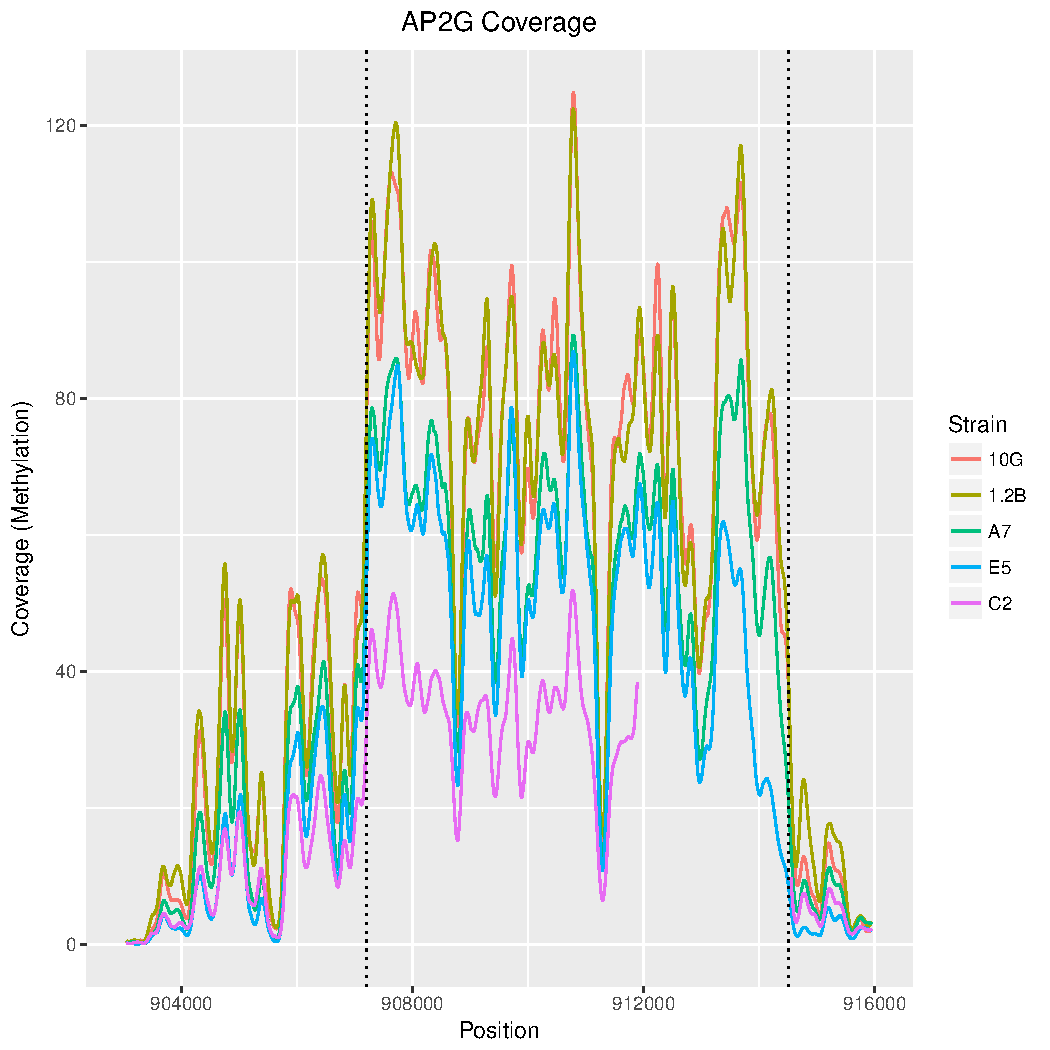
\includegraphics[width=1\linewidth]{figure/plot_coverage-1} 

\end{knitrout}
\clearpage
\subsection{Coverage Normalitzat}
\begin{knitrout}
\definecolor{shadecolor}{rgb}{0.969, 0.969, 0.969}\color{fgcolor}
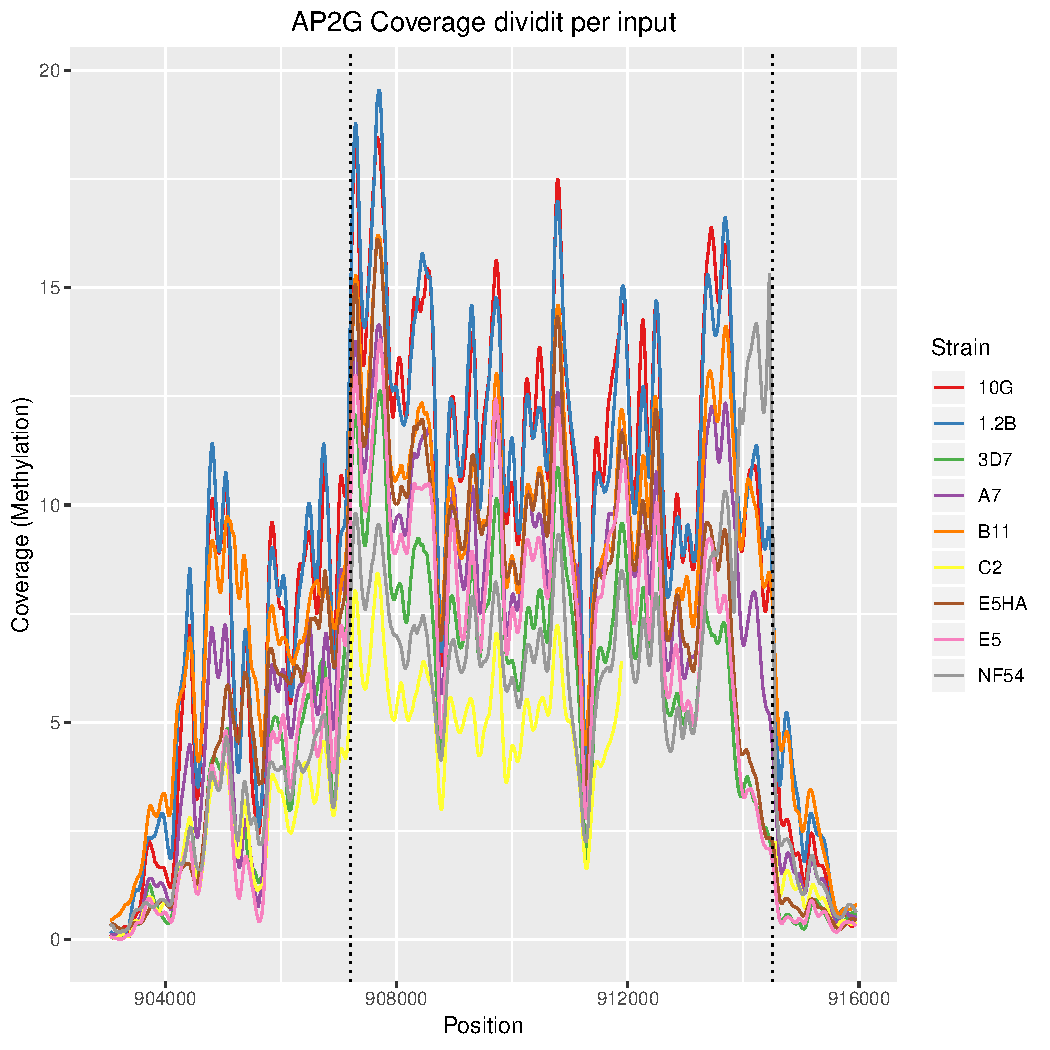
\includegraphics[width=1\linewidth]{figure/plot_norm_cov-1} 

\end{knitrout}
\clearpage
\subsection{Coverage "Equalitzat"}
\begin{knitrout}
\definecolor{shadecolor}{rgb}{0.969, 0.969, 0.969}\color{fgcolor}
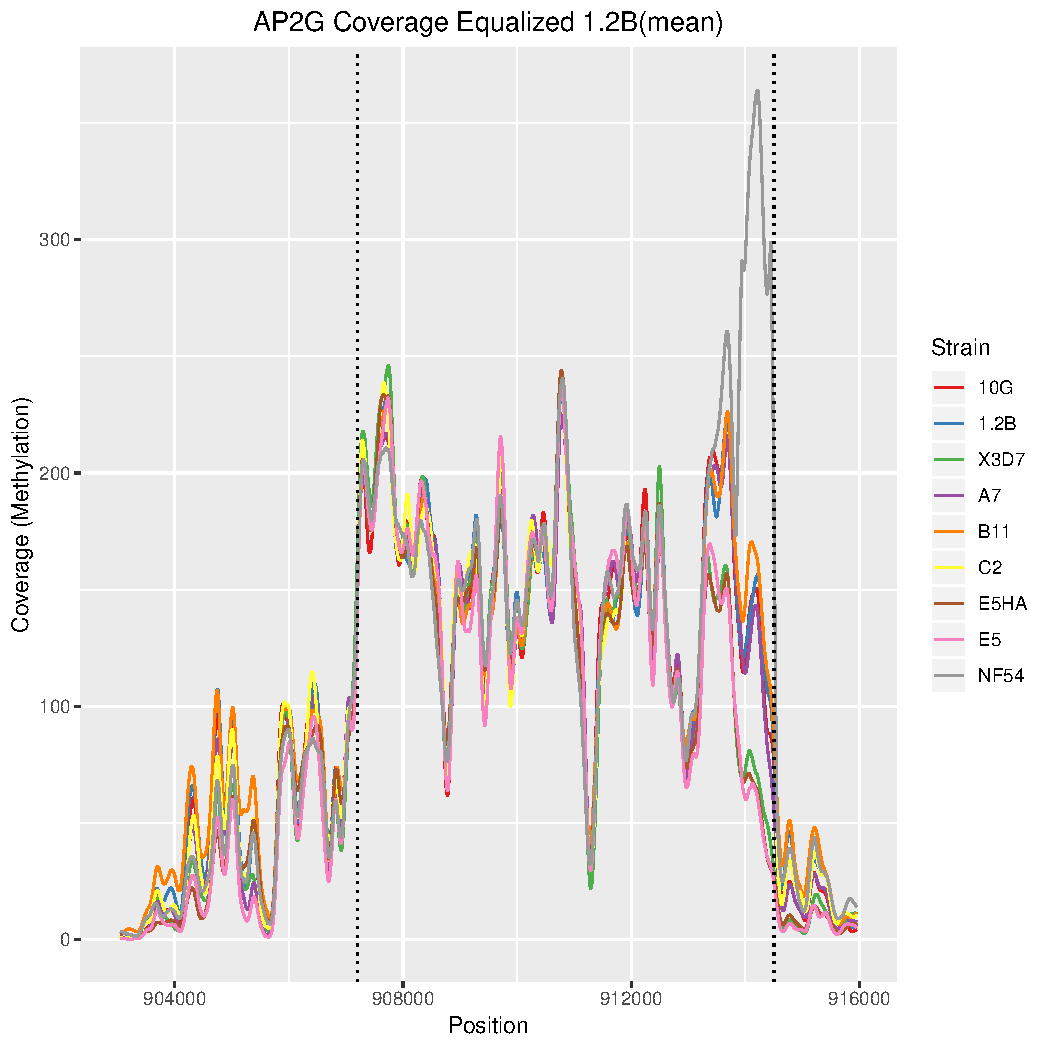
\includegraphics[width=1\linewidth]{figure/plot_equalizedCov-1} 

\end{knitrout}
\clearpage
\subsection{Coverage "Equalitzat": 10G vs 1.2B}
\begin{knitrout}
\definecolor{shadecolor}{rgb}{0.969, 0.969, 0.969}\color{fgcolor}
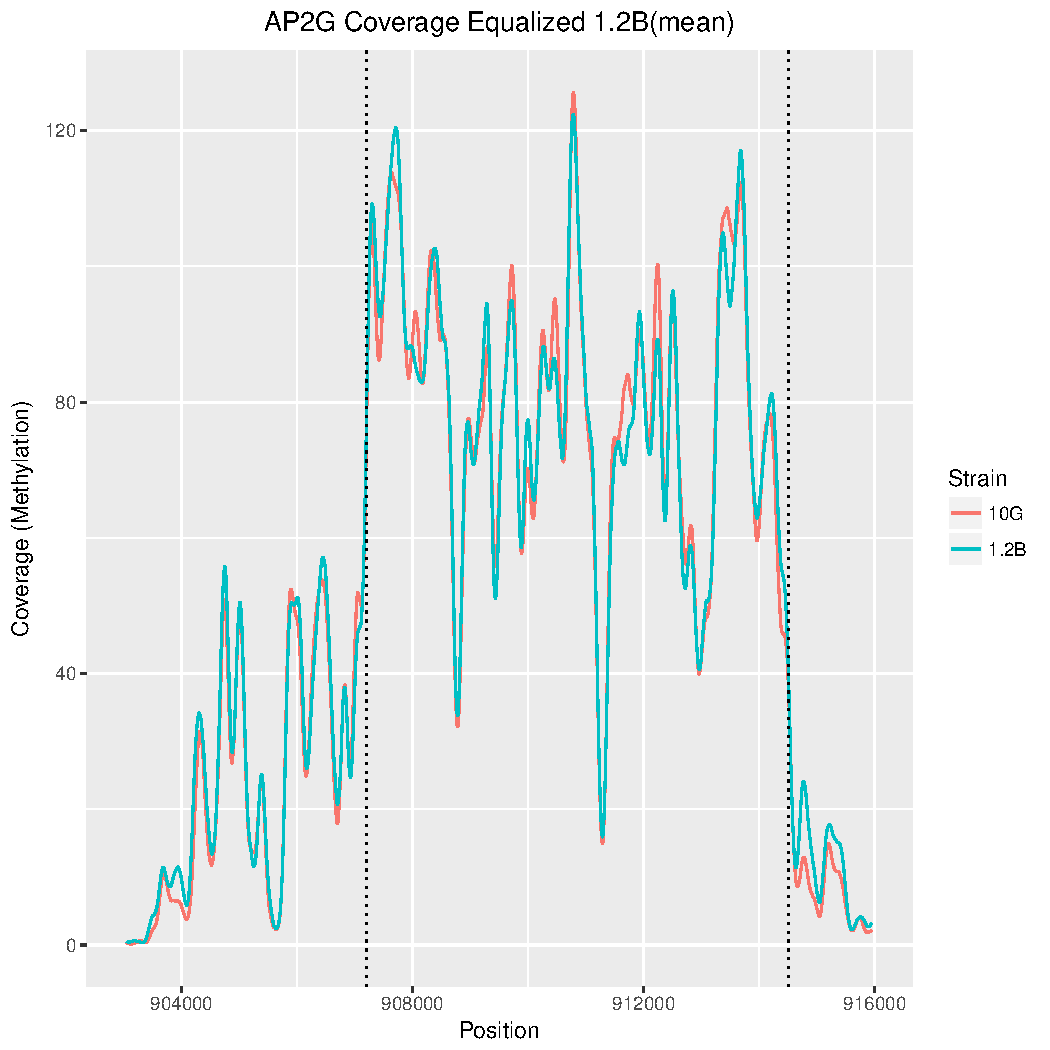
\includegraphics[width=1\linewidth]{figure/plot_equalizedCov_10vs1_2-1} 

\end{knitrout}
\clearpage
\subsection{Coverage "Equalitzat": 10G, E5, A7}
\begin{knitrout}
\definecolor{shadecolor}{rgb}{0.969, 0.969, 0.969}\color{fgcolor}
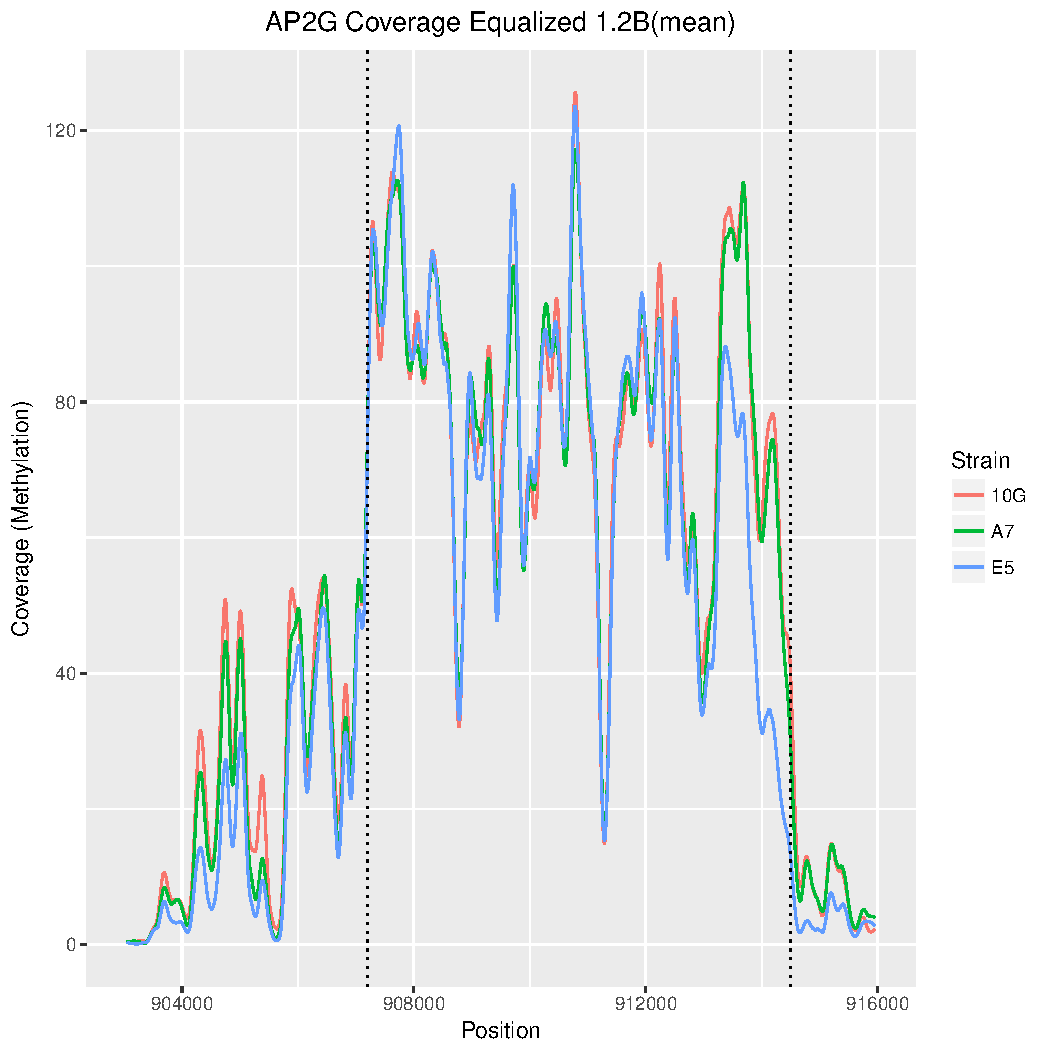
\includegraphics[width=1\linewidth]{figure/plot_equalizedCov_3sample-1} 

\end{knitrout}
\clearpage
\subsection{Coverage Normalitzat i "Equalitzat"}
\begin{knitrout}
\definecolor{shadecolor}{rgb}{0.969, 0.969, 0.969}\color{fgcolor}
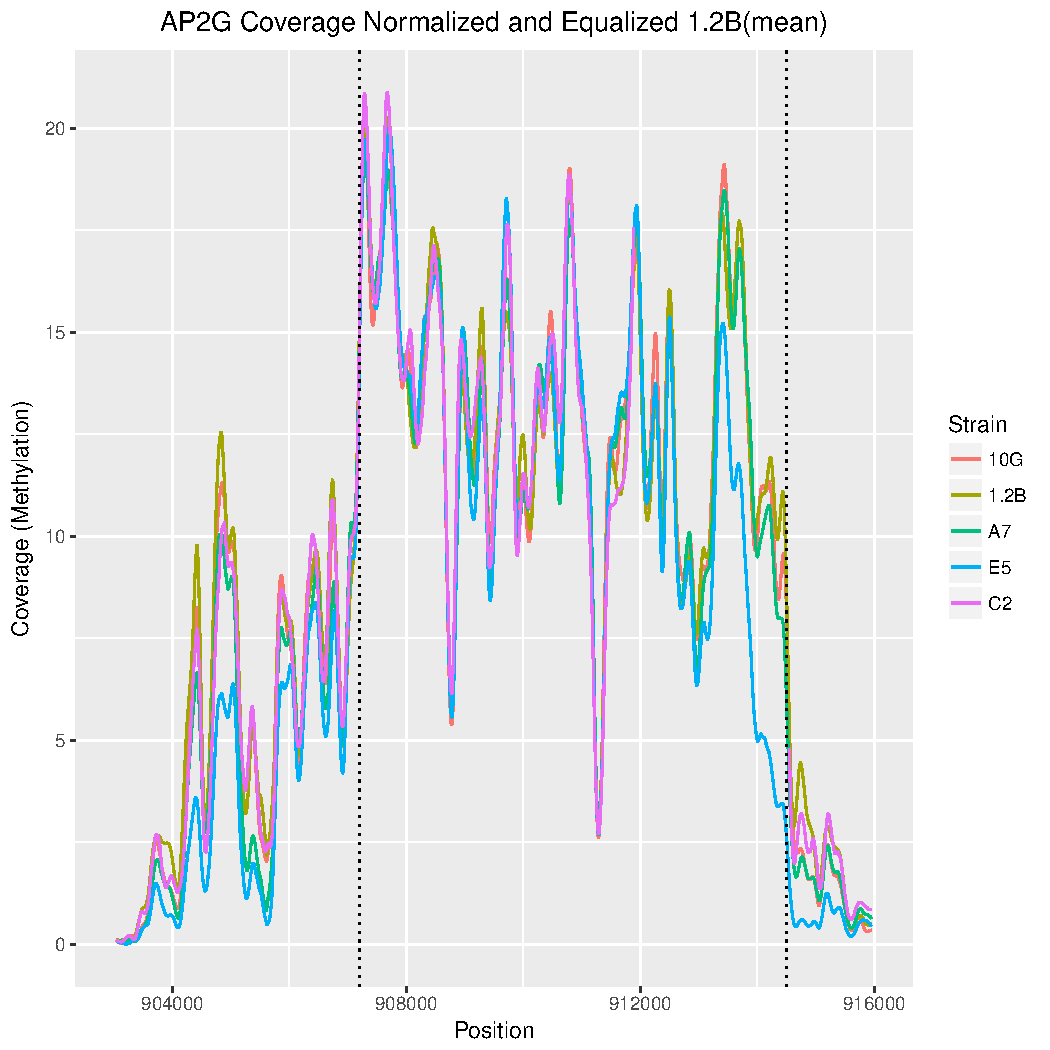
\includegraphics[width=1\linewidth]{figure/plot_NormequalizedCov-1} 

\end{knitrout}
\clearpage
\subsection{Coverage Normalitzat i "Equalitzat": 10G, 1.2B}
\begin{knitrout}
\definecolor{shadecolor}{rgb}{0.969, 0.969, 0.969}\color{fgcolor}
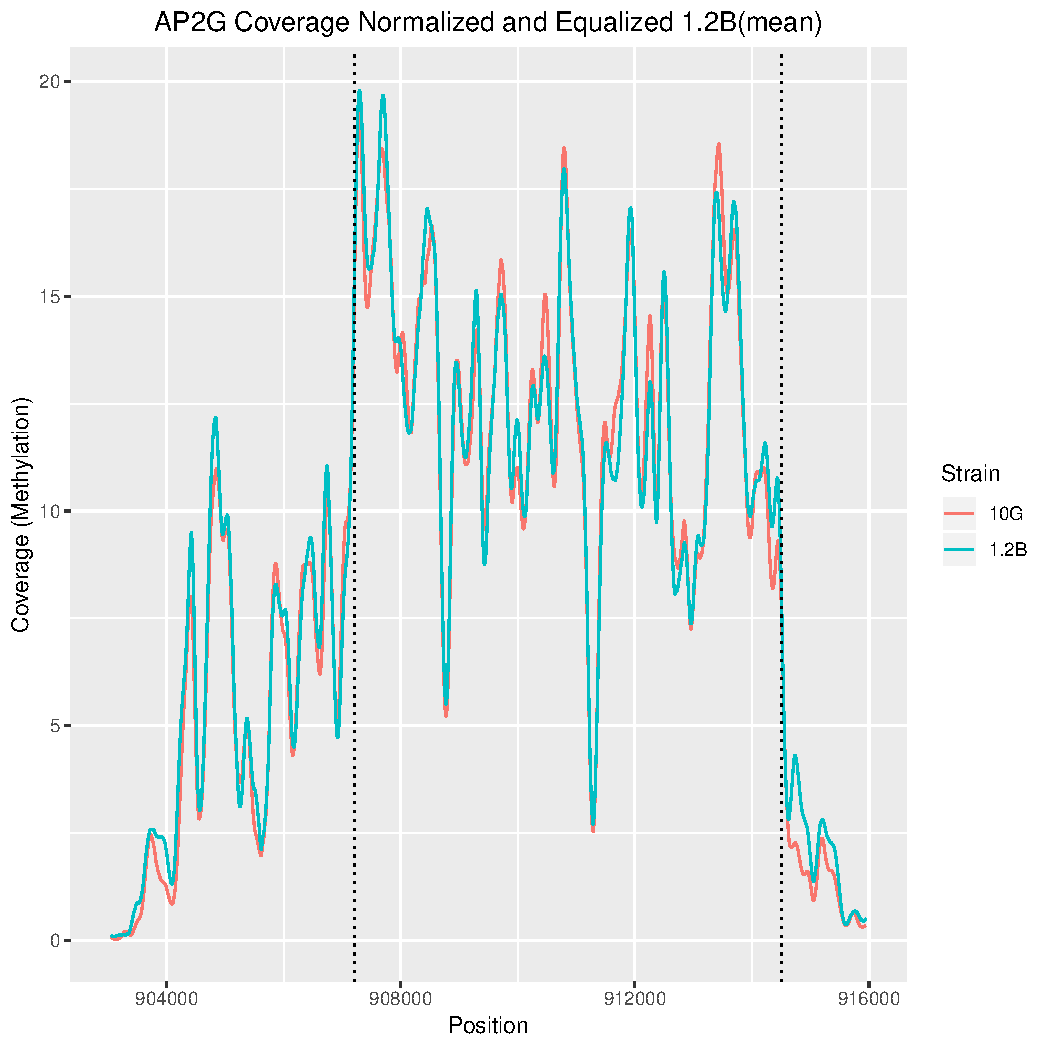
\includegraphics[width=1\linewidth]{figure/plot_NromequalizedCov_10vs1_2-1} 

\end{knitrout}
\clearpage
\subsection{Coverage Normalitzat i "Equalitzat": 10G, E5, A7}
\begin{knitrout}
\definecolor{shadecolor}{rgb}{0.969, 0.969, 0.969}\color{fgcolor}
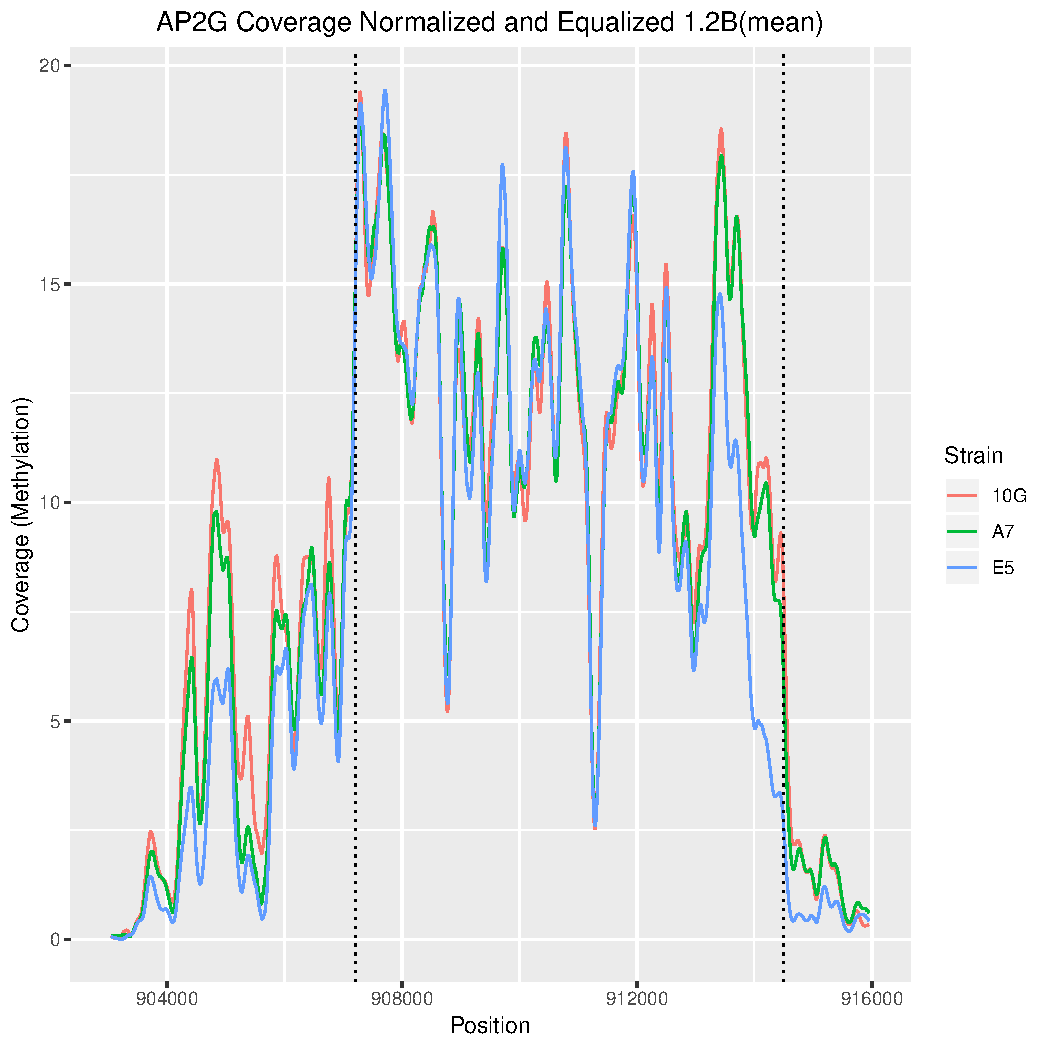
\includegraphics[width=1\linewidth]{figure/plot_NromequalizedCov_3sample-1} 

\end{knitrout}
\clearpage
\subsection{Coverage Normalitzat a regió 5'}
\begin{knitrout}
\definecolor{shadecolor}{rgb}{0.969, 0.969, 0.969}\color{fgcolor}
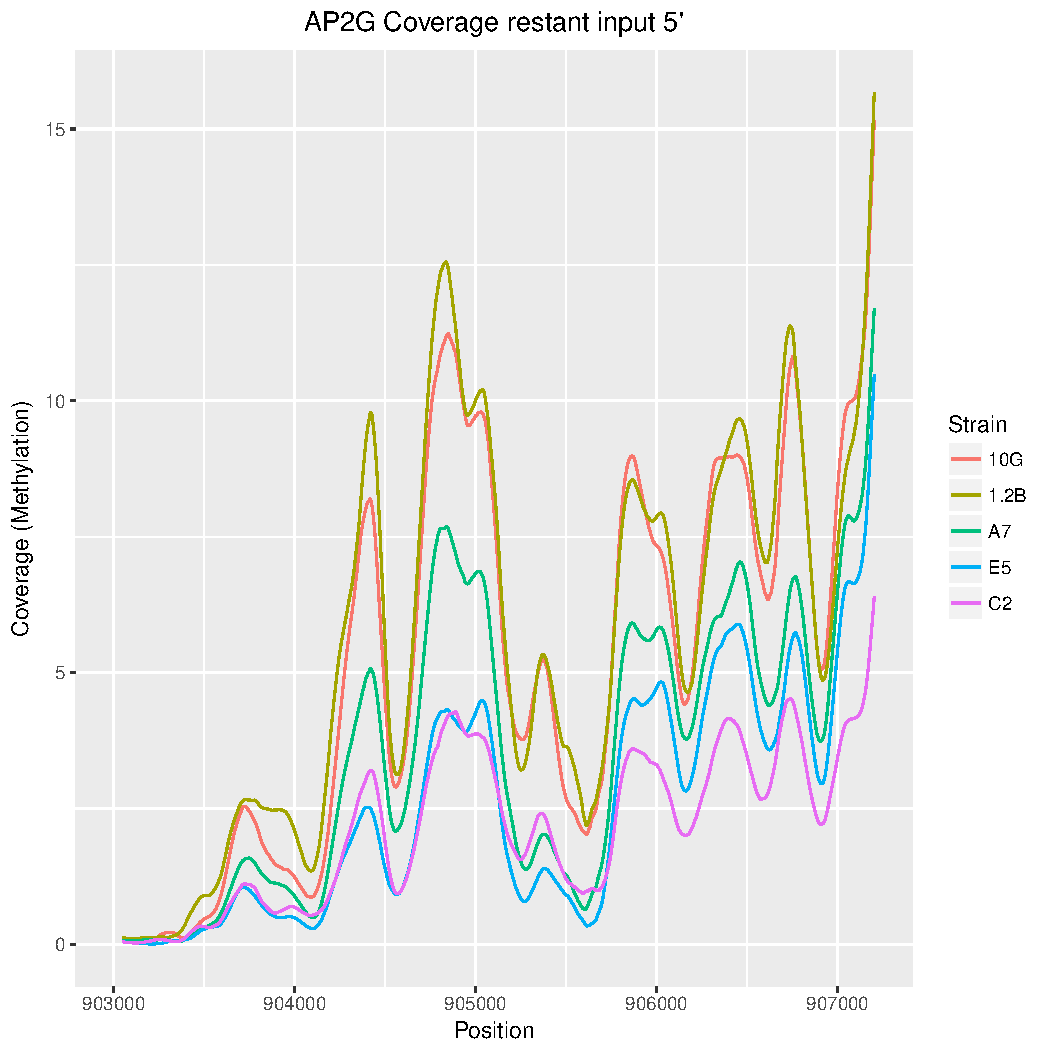
\includegraphics[width=1\linewidth]{figure/plot_norm_cov_5-1} 

\end{knitrout}
\clearpage
\subsection{Coverage Acetilació}
\begin{knitrout}
\definecolor{shadecolor}{rgb}{0.969, 0.969, 0.969}\color{fgcolor}
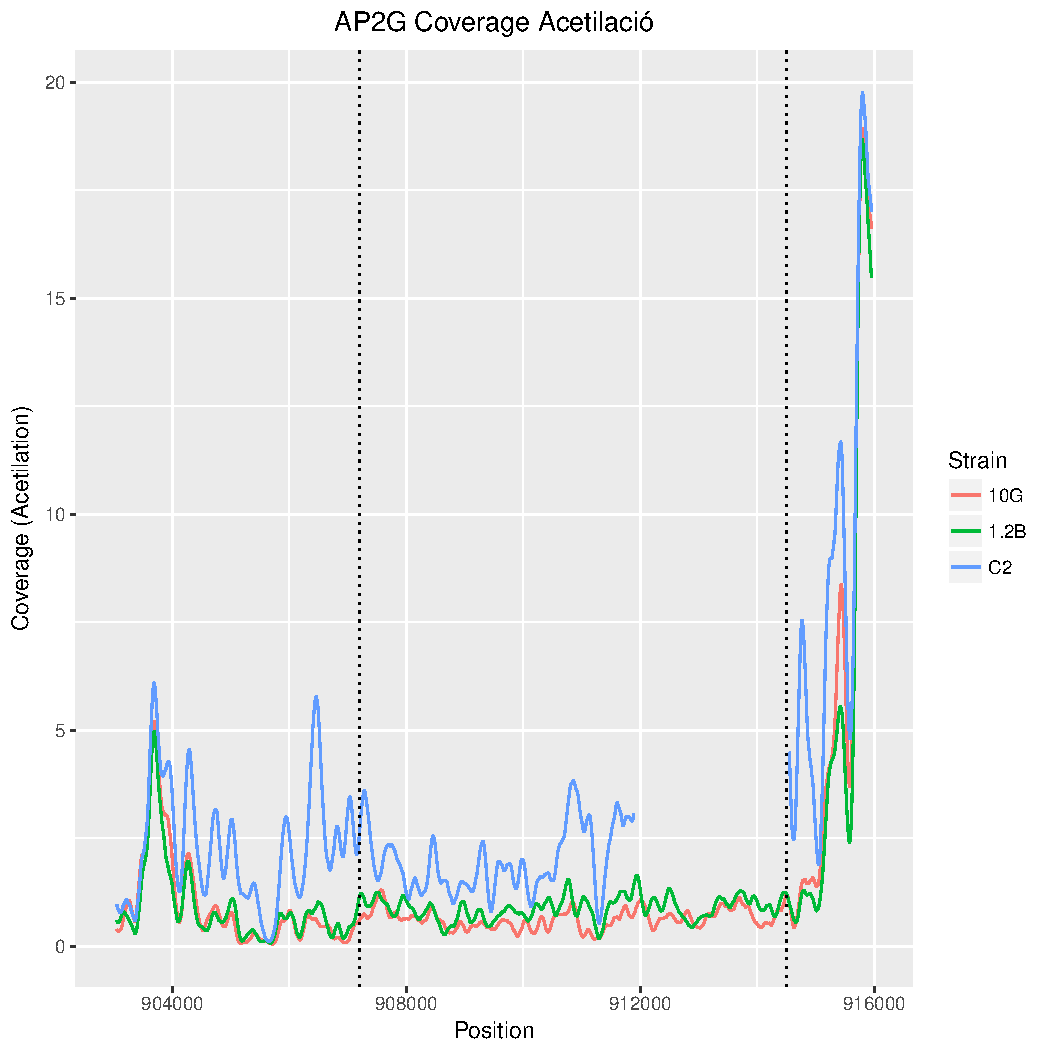
\includegraphics[width=1\linewidth]{figure/plot_ac-1} 

\end{knitrout}
\clearpage
\subsection{Coverage Acetilació a 5'}
\begin{knitrout}
\definecolor{shadecolor}{rgb}{0.969, 0.969, 0.969}\color{fgcolor}
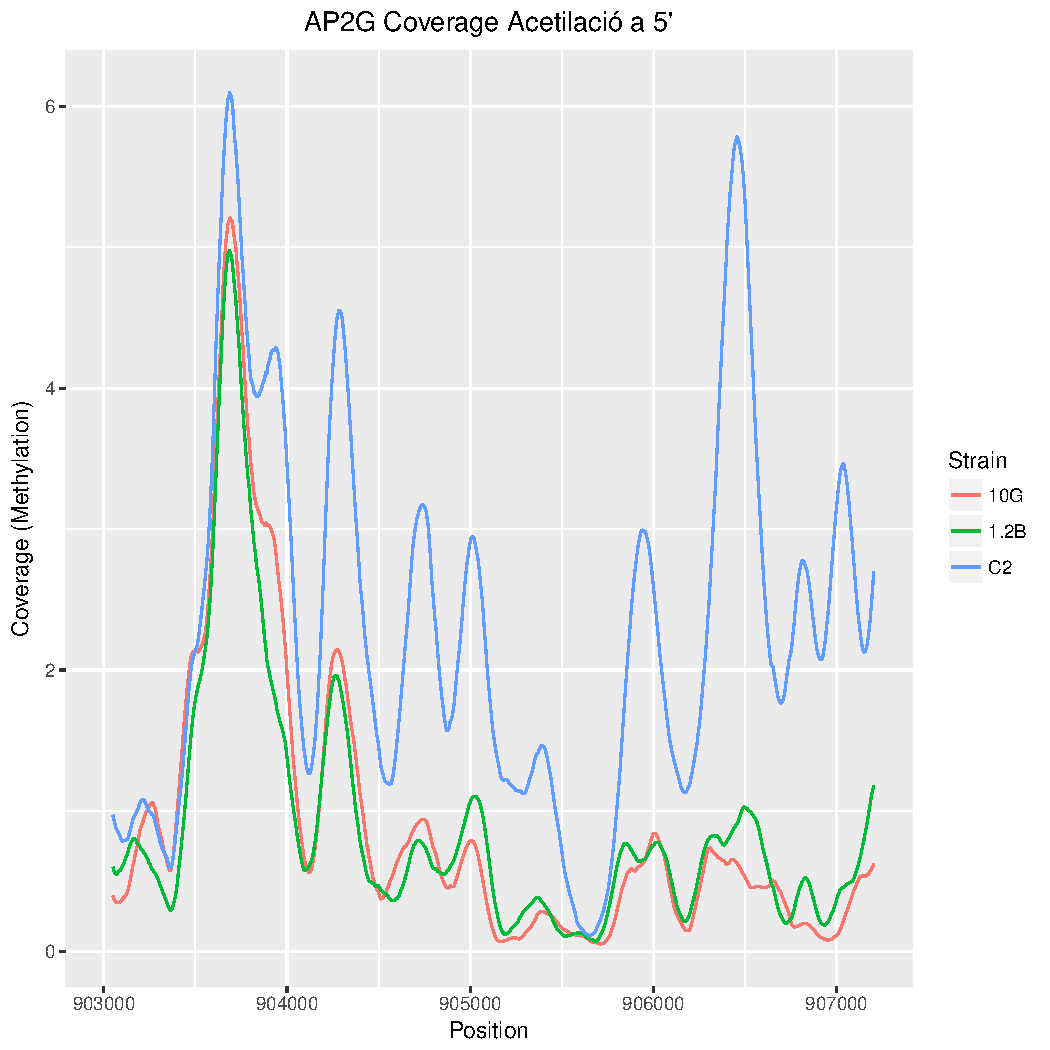
\includegraphics[width=1\linewidth]{figure/plot_ac_5-1} 

\end{knitrout}
\clearpage
\subsection{Acetilació / Metilació (normalitzat per input)}
\begin{knitrout}
\definecolor{shadecolor}{rgb}{0.969, 0.969, 0.969}\color{fgcolor}
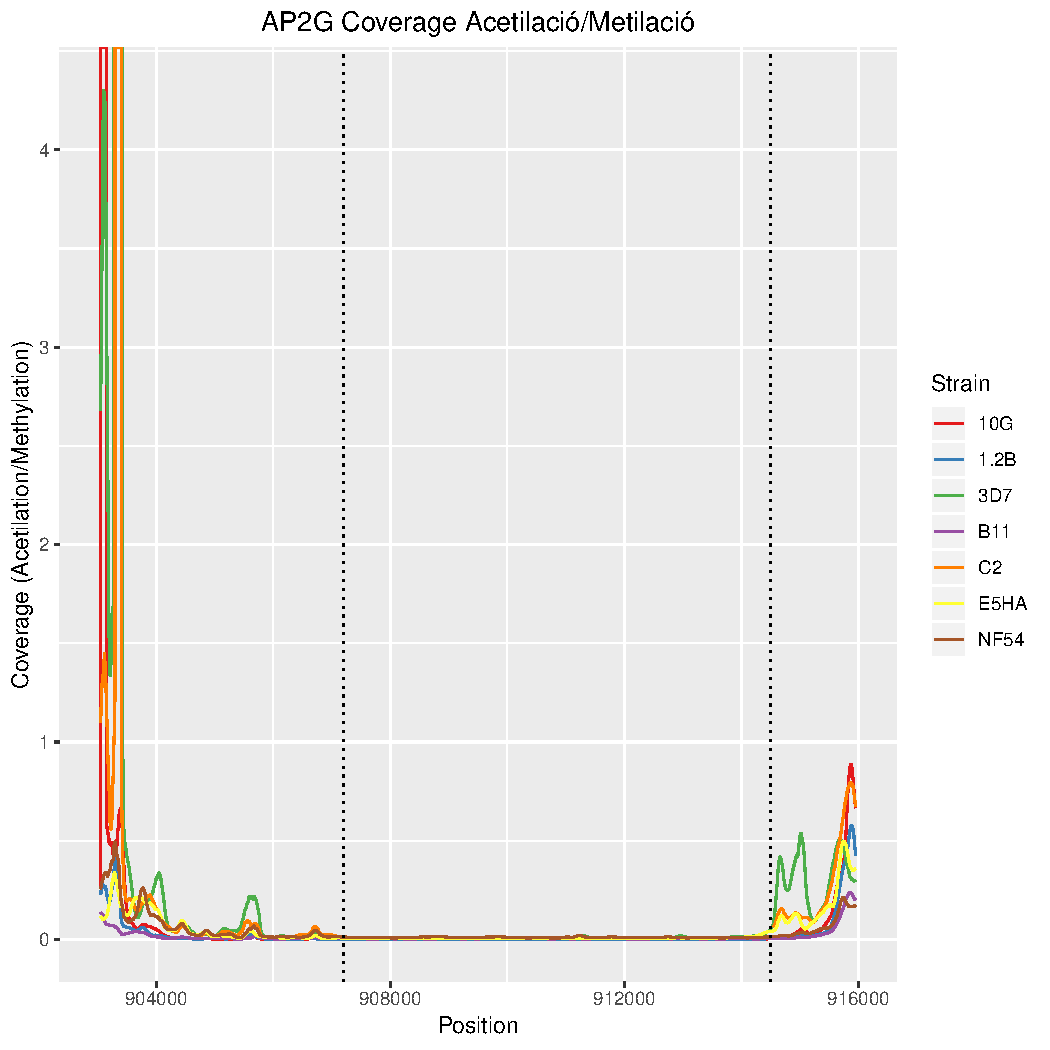
\includegraphics[width=1\linewidth]{figure/Ac_Met-1} 

\end{knitrout}
\clearpage
\subsection{Metilació / Acetilació (normalitzat per input)}
\begin{knitrout}
\definecolor{shadecolor}{rgb}{0.969, 0.969, 0.969}\color{fgcolor}
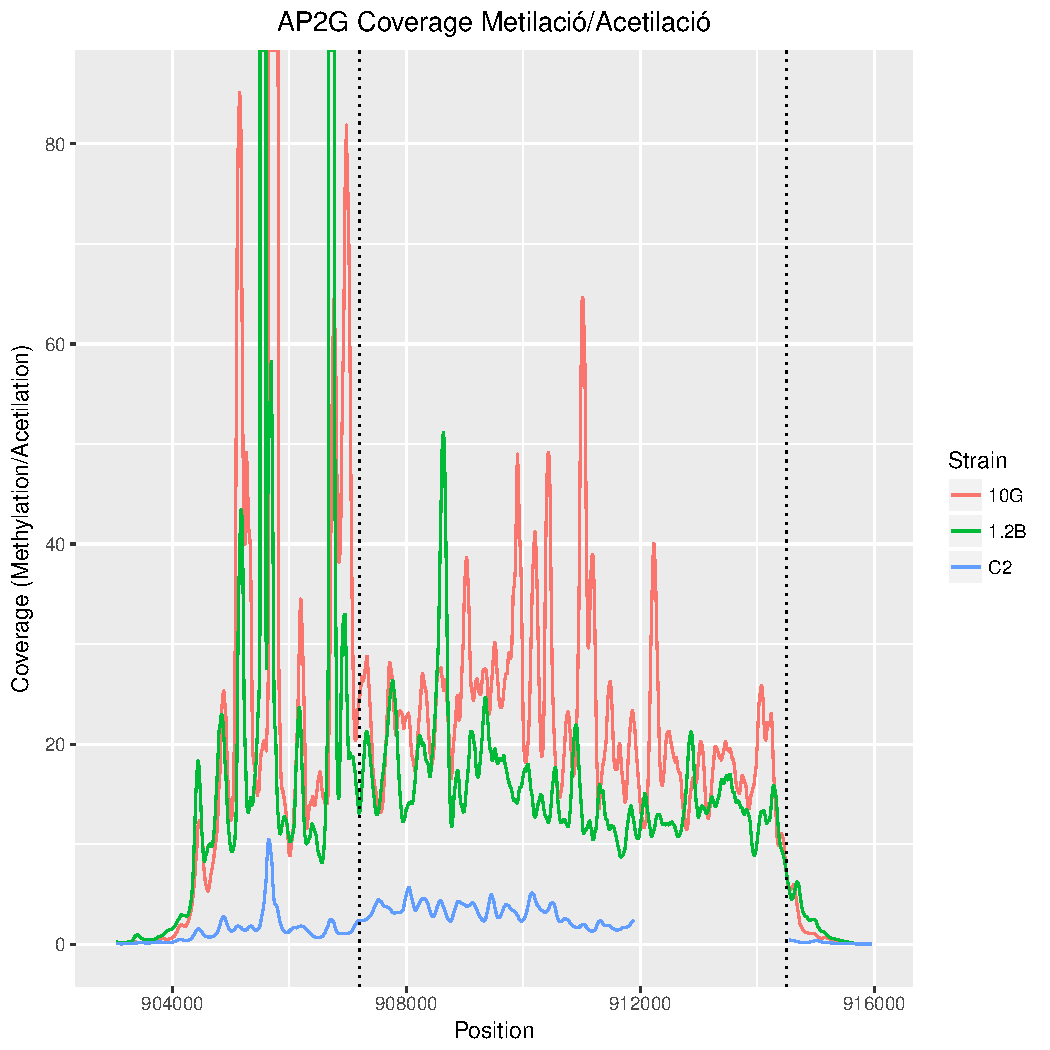
\includegraphics[width=1\linewidth]{figure/Met_Ac-1} 

\end{knitrout}

\end{document}
